\documentclass[12pt]{article}
\usepackage[utf8x]{inputenc}
\usepackage[hebrew,english]{babel}
\usepackage{culmus}
\usepackage[yyyymmdd]{datetime}
\usepackage{amsmath,amssymb,amsthm}
\usepackage{graphicx}
\usepackage{textcomp}
\usepackage{mdframed}
\usepackage{lipsum}
%general:
%Box and color definitions:
%--------------------------
\newenvironment{ColorBoxedminipage}
{\begin{minipage}} {\end{minipage}}
%{\begin{Sbox}\begin{minipage}}
%{\end{minipage}\end{Sbox}\fcolorbox{Blue}{White}{\TheSbox}}

%General definitions:
%-------------------
\newcommand{\etal}{{\em {et al.}}}
\newcommand{\B}[1]{\mathbf{#1}}
\newcommand{\df}{\triangleq}
\newcommand{\norm}[1]{\left\Vert#1\right\Vert}
\newcommand{\abs}[1]{\left\vert#1\right\vert}
\newcommand{\RE}{\operatorname{Re}}
\newcommand{\IM}{\operatorname{Im}}
\newcommand{\sgma}[3]{\sum\limits_{{#1}={#2}}^{#3}}
\newcommand{\Brace}[1]{\left\{{#1}\right\}} %Braces
\newcommand{\Brack}[1]{\left({#1}\right)} %Brackets
\newcommand{\sBrack}[1]{\left[{#1}\right]} %square Brackets

%\newcommand{\ip}[2]{{\langle{#1},{#2}\rangle}} %inner-product
\newcommand{\ipLW}[3]{{\langle{#1},{#2}\rangle}_{{#3}}} %weighted inner-product

\newcommand{\Tr}[1]{Tr\Brack{#1}}
\newcommand{\Mtr}[2] %short notation for 2x1 Matrix.
{\begin{bmatrix}
  #1 \\
  #2
\end{bmatrix}}
\newcommand{\cMtr}[2] %short notation for 2x1 Matrix with curves.
{\left(
\begin{array}{c}
    {#1} \\
    {#2} \\
\end{array}
\right)}
\newcommand{\Mtrs}[2] %short notation for 2x1 Matrix star (adjoint)
{\begin{bmatrix}
  #1 &
  #2
\end{bmatrix}}
\newcommand{\Mtrt}[3] %short notation for 3x1 Matrix.
{\begin{bmatrix}
  #1 \\
  #2 \\
  #3
\end{bmatrix}}

\newcommand{\Cases}[4]{
\left\{
\begin{tabular}{lcl}
    $#1$ & $=$ & $#2$\\
    $#3$     & $=$ & $#4$
\end{tabular}
\right. }

\newcommand{\und}{\underline} %How lazy can I get?
\newcommand{\ovr}{\overline}
\newcommand{\conj}[1]{{#1}^\ast} %Conjugation


\newcommand{\er}[1]{{(\ref{#1})}} %equation reference

\newtheorem{Lemma}{Lemma}{}
\newtheorem{Prop}{Proposition}{}
\newtheorem{theorem}{Theorem}{}


\newenvironment{alg}[5]
{
\begin{figure}[htbp]
\begin{center}
\fbox{
  \begin{ColorBoxedminipage}{13cm}
%    \leftline{\color{Black}\bf {#1}}
    {#4}
   \end{ColorBoxedminipage}
   }
\end{center}
  \bcaptionff{#1}{#2}{}{#3}
  \label{#5}
\end{figure}
}{}

%Just body, caption and label.
\newenvironment{algo}[3]
{
\begin{figure}[htbp]
\begin{center}
\fbox{
  \begin{ColorBoxedminipage}{7.5cm}
%    \leftline{\color{Black}\bf {#1}}
    {#1}
   \end{ColorBoxedminipage}
   }
\end{center}
  \caption{#2}
  \label{#3}
\end{figure}
}{}

\newenvironment{BOX}[1]
{
\begin{center}
\fbox{
  \begin{ColorBoxedminipage}{16cm}
%    \leftline{\color{Black}\bf {#1}}
    {#1}
   \end{ColorBoxedminipage}
   }
\end{center}
}{}

\newcommand\vecnot[1]{\boldsymbol{#1}}
\newcommand\optvecnot[1]{\vecnot{#1}_{opt}}

\usepackage{amsmath}
\DeclareMathOperator*{\argmax}{arg\,max}
\DeclareMathOperator*{\argmin}{arg\,min}

%Configuration-------------------------------------------------------------
\setlength{\parskip}{0.2cm}
\setlength{\parindent}{0cm}
\addto{\captionshebrew}{
    \renewcommand{\refname}{Bibliography}
    \renewcommand{\contentsname}{Table of Contents}
}
\newcommand{\printdate}[3]{{%
\day=#1\relax\month=#2\relax\year=#3\relax\today}}

\title{
\begin{otherlanguage}{hebrew}
עדכון התקדמות במחקר
\end{otherlanguage}
\\
Research status update
}
\author{
\\Yehezkel Karo Itay
}
\begin{document}
\maketitle
\section*{Introduction}
This document's purpose is to serve as a constantly updated elaborated presentation of the research's current status.
The research presentations will rely on its content.
\section{Research motivation}

Uniform linear array (ULA) processing in the spatial domain is similar to time domain finite-impulse-response (FIR) filtering (e.g. \cite{van1988beamforming}).
The similarity arises because temporal FIR's input is composed of equally time-spaced samples and the ULA's input is obtained from equally spatially-spaced samples of the impinging wavefront.
Both temporal FIR and ULA filtering assign weights to each sample in order to achieve a desired temporal/spatial response.
From time domain filter design theory, it is well known that infinite impulse response (IIR) filters attain certain advantages over FIR filtering.
A natural question to consider is ``what is the array structure in spatial domain which is analogous to IIR filtering in the time domain?''.
The motivation for finding an IIR equivalent in the spatial domain is obvious:
\begin{itemize}
\item
{
Increased degrees of freedom over conventional array processing to control the array response.
}
\item
{
Substantially lower number of taps (smaller number of array elements and reduced array aperture) is required for obtaining a desired response in comparison to an FIR based design. This, naturally, results in cost-efficient array.
}
\end{itemize}
Our work was motivated from a prediction that a spatial-IIR should be achievable and later, after exposing to Wen's work \cite{FuxiARRAYMODEL} based on it.

\section*{Previous suggested method Discussion}

\subsection*{approximating the delay between sensors' input ($ \tau_{\theta} $) with DOA estimation}
\begin{figure}
\begin{center}
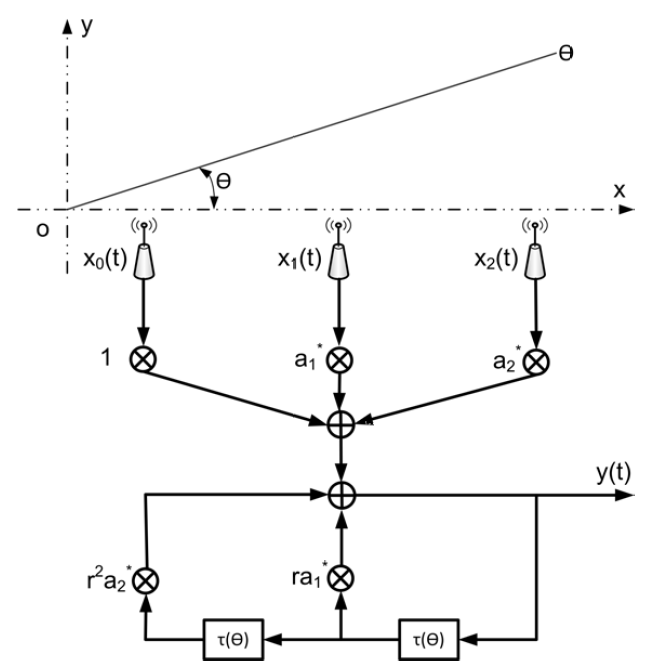
\includegraphics[width=.4\textwidth]{Media/WenFirstSuggestedMethod.PNG}
\caption{Wen's first suggested method - DOA estimation and approximated synthetic feedback delay.}
\end{center}
\label{fig:WenTauApproxDOAEst}
\end{figure}
As can be seen in fig.\ref{fig:WenTauApproxDOAEst}, this method merely enables single-speaker scenarios and while not simulated or proved, we assume it is very sensitive to DOA estimation errors. Heuristically, to understand the DOA estimation high sensitivity, one can imagine an IIR digital filter whose recursive shift-delay part doesn't generate a similar delay and the designer is not aware of this fact.

\subsection*{Using multiple ULA subsets to create a spatially diverse spatial-FIR outputs}
\begin{figure}
\begin{center}
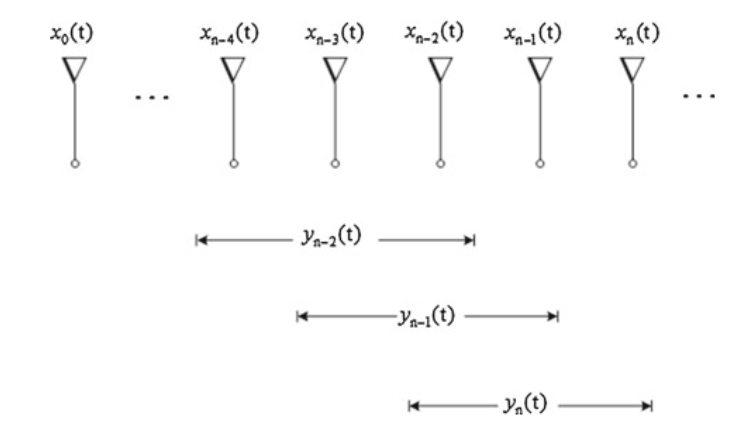
\includegraphics[width=.4\textwidth]{Media/SpatialIIR_SubArrays.PNG}
\caption{Wen's second suggested method - Shifted sub arrays to emulate IIR filter}
\label{fig:ShiftedSubArraysWen}
\end{center}
\end{figure}
Though this method actually achieves spatial diverse spatial-FIR (smaller-aperture array) outputs (fig.\ref{fig:ShiftedSubArraysWen}), it lacks the IIR basic feature of infinite system memory and when practically examined, it reveals as a complicated way of designing a spatial-FIR with the same number of DOF (degrees of freedom) as a regular delay-and-sum beam-formers.

\subsection*{Spatio-temporal 2D plane-waves filtering}
\begin{figure}
\begin{center}
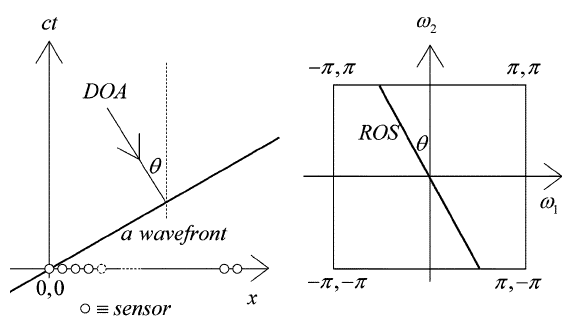
\includegraphics[width=.4\textwidth]{Media/SpatioTemporalPlaneWave.PNG}
\caption{Spatio-temporal representation of plane wave}
\label{fig:SpatioTemporalPlaneWave}
\end{center}
\end{figure}
\begin{figure}
\begin{center}
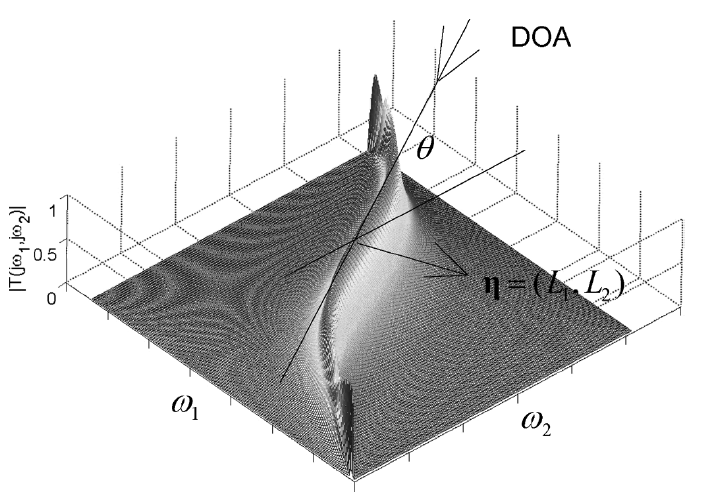
\includegraphics[width=.4\textwidth]{Media/SpatioTemporalPlaneWavePracticalFilter.PNG}
\caption{Practical spatio-temporal 2D plane-wave filter.}
\label{fig:SpatioTemporalPlaneWavePracticalFilter}
\end{center}
\end{figure}
Additional works \cite{Madanayake2008ABeamformer,Madanayake2009SystolicWDFs,Madanayake2008AFilters,Bruton2003Three-dimensionalBanks,Ward1986ABeamforming,Joshi2012SynthesisApplications} consider a different approach of 2-D spatio-temporal filtering. In particular, the wavefront is viewed as a two dimensional signal, and the processing is done by performing IIR filtering in the time domain, but only FIR filtering (using a finite number of sensors) is performed in the spatial domain.
As can be seen in \cite{Bruton2003Three-dimensionalBanks} (and in fig.\ref{fig:SpatioTemporalPlaneWavePracticalFilter}), due to the filter's inherent cyclic characteristics, the obtained 2-D filter is not ideal, causing imperfections in the overall spatial response.

\section*{Our suggested architecture for spatial-IIR beam-former}

\begin{figure}[!ht]
\begin{center}
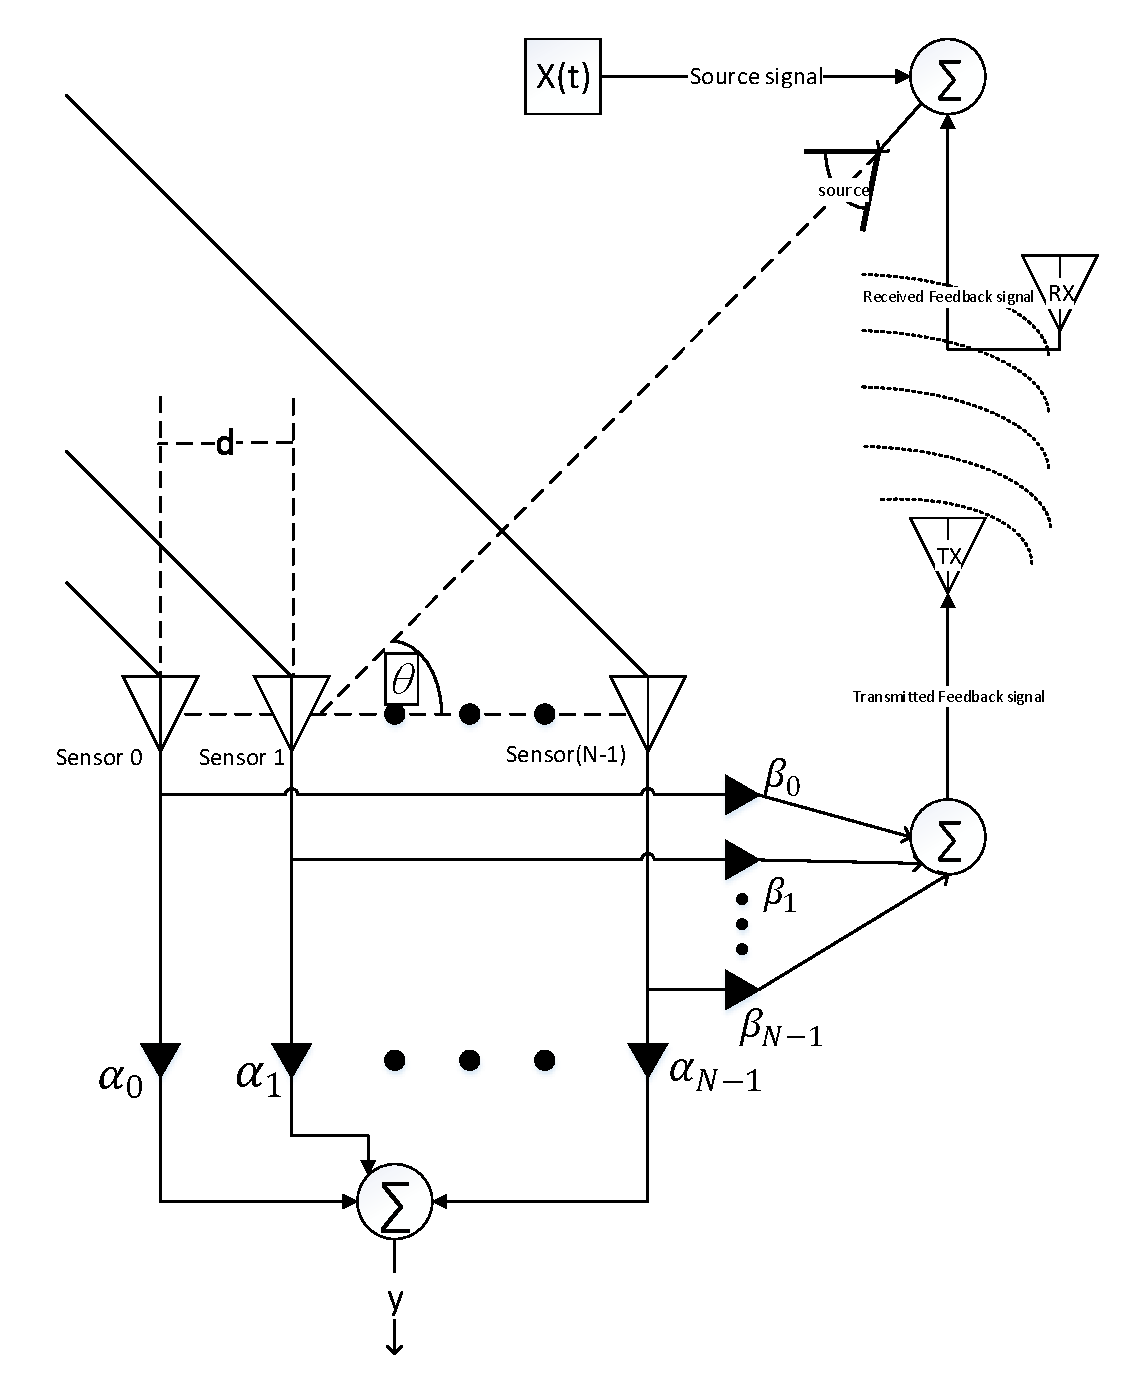
\includegraphics[width=0.7\textwidth]{./Media/SpatialIIR-diagram/SpatialIIR_VER4.pdf}
\caption
{
The proposed system: A far field source is received by an array. 
The received signal is also retransmitted back to the source. 
The latter has a transponder which feeds the signal back to the array.
}
\label{fig:SignalModel}
\end{center}
\end{figure}
By creating the suggested setup (fig.\ref{fig:SignalModel}), we aim to achieve a spatial-IIR which was previously discussed. 
Assume a far field source with signal $x(t)$. 
The resulting wavefront, with direction of arrival (DOA) $\theta$, is received by an array. 
For simplicity, we first assume a ULA, with elements spacing $d$. A weight and sum beamformer, with weights $\beta_n,\;n=0,...,N-1$  is used to retransmit the signal back to the source point. 
The retransmission can be conducted after RF modulation, or possibly acoustically, in the context of acoustical signal processing. 
As this cooperative source has a transponder, the obtained feedback signal, together with its own source signal $x(t)$ are summed up, and collected again by the array. 
A weight and sum beam-former, with weights $\alpha_n,\;n=0,...,N-1$ is used prior to generating the final output signal $y(t)$.
It can be proved that our suggested architecture, for a single-speaker scenario actually implements a \textbf{spatial-only} controllable transfer function
$$
\ensuremath{
y_{\theta}^{\mathcal{F}}(\omega) 
=
\frac
{
\vecnot{\alpha}^{T}
\vecnot{d}_{\theta}
exp\left(-j\tau\right)
}
{
1
-
\vecnot{\beta}^{T}\vecnot{d}_{\theta}
exp\left(-j\tau\right)
}
x^{\mathcal{F}}(\omega)
}
$$
where $ x^{\mathcal{F}}(\omega) $ is the source's signal Fourier transform, which travels in the medium with propagation speed of $ c $, $ \theta $ is the DOA, $ \tau_{pd}$ is the propagation delay from the source to the reference sensor, $ \tau_{tx} $ is the feedback transmission delay, $\vecnot{d}_{\theta}$ is the steering vector with n$ ^{th} $ element $e^{-j\omega \tau_{n,\theta}}$, $ \tau_{n,\theta}=n\frac{d\cos(\theta)}{c} $ is the sensor's location related delay (in case of ULA), and $\vecnot{\alpha,\beta}$ are the controllable coefficient vectors.
$^{T}$ stands for the transpose operator.
\\
Ideally, when all parameters are known we can design a wanted IIR filter 
$ 
H_{wanted}(\theta) = \frac{\vecnot{\alpha}_{wanted}^{T}\vecnot{d}_{\theta}}{\vecnot{\beta}_{wanted}^{T}\vecnot{d}_{\theta}}
$ 
and adjust 
$
\vecnot{\alpha,\beta}
$ 
so that 
$ 
\vecnot{\alpha}^{T}\vecnot{d}_{\theta}e^{-j\omega \tau_{pd}} = \vecnot{\alpha}_{wanted}^{T}\vecnot{d}_{\theta} 
$ 
and 
$ 1 - \vecnot{\beta}^{T}\vecnot{d}_{\theta}e^{-j\omega (\tau_{pd}+\tau_{tx})} = \vecnot{\beta}_{wanted}^{T}\vecnot{d}_{\theta} 
$
but in a practical scenarios, where some uncertainties arise we experience some issues that will be discussed in the next section.

\section*{Transfer function practical issues}

\subsection*{High sensitivity to object range uncertainty}

A closer investigation of the transfer function's denominator reveals two components
\begin{itemize}
\item
{
$ \mathbf{ 1 } $
\\
which cannot be controlled.
}
\item
{
$
\mathbf{
\vecnot{\beta}^{T}\vecnot{d}_{\theta}e^{-j\omega (\tau_{pd}+\tau_{tx})} 
}
$
\\
which can be partially controlled. The amplitude is fully controllable but the phase is influenced by the $ \tau_{pd} $ (the object's range). 
}
\end{itemize}
\begin{figure}[!ht]
\begin{center}
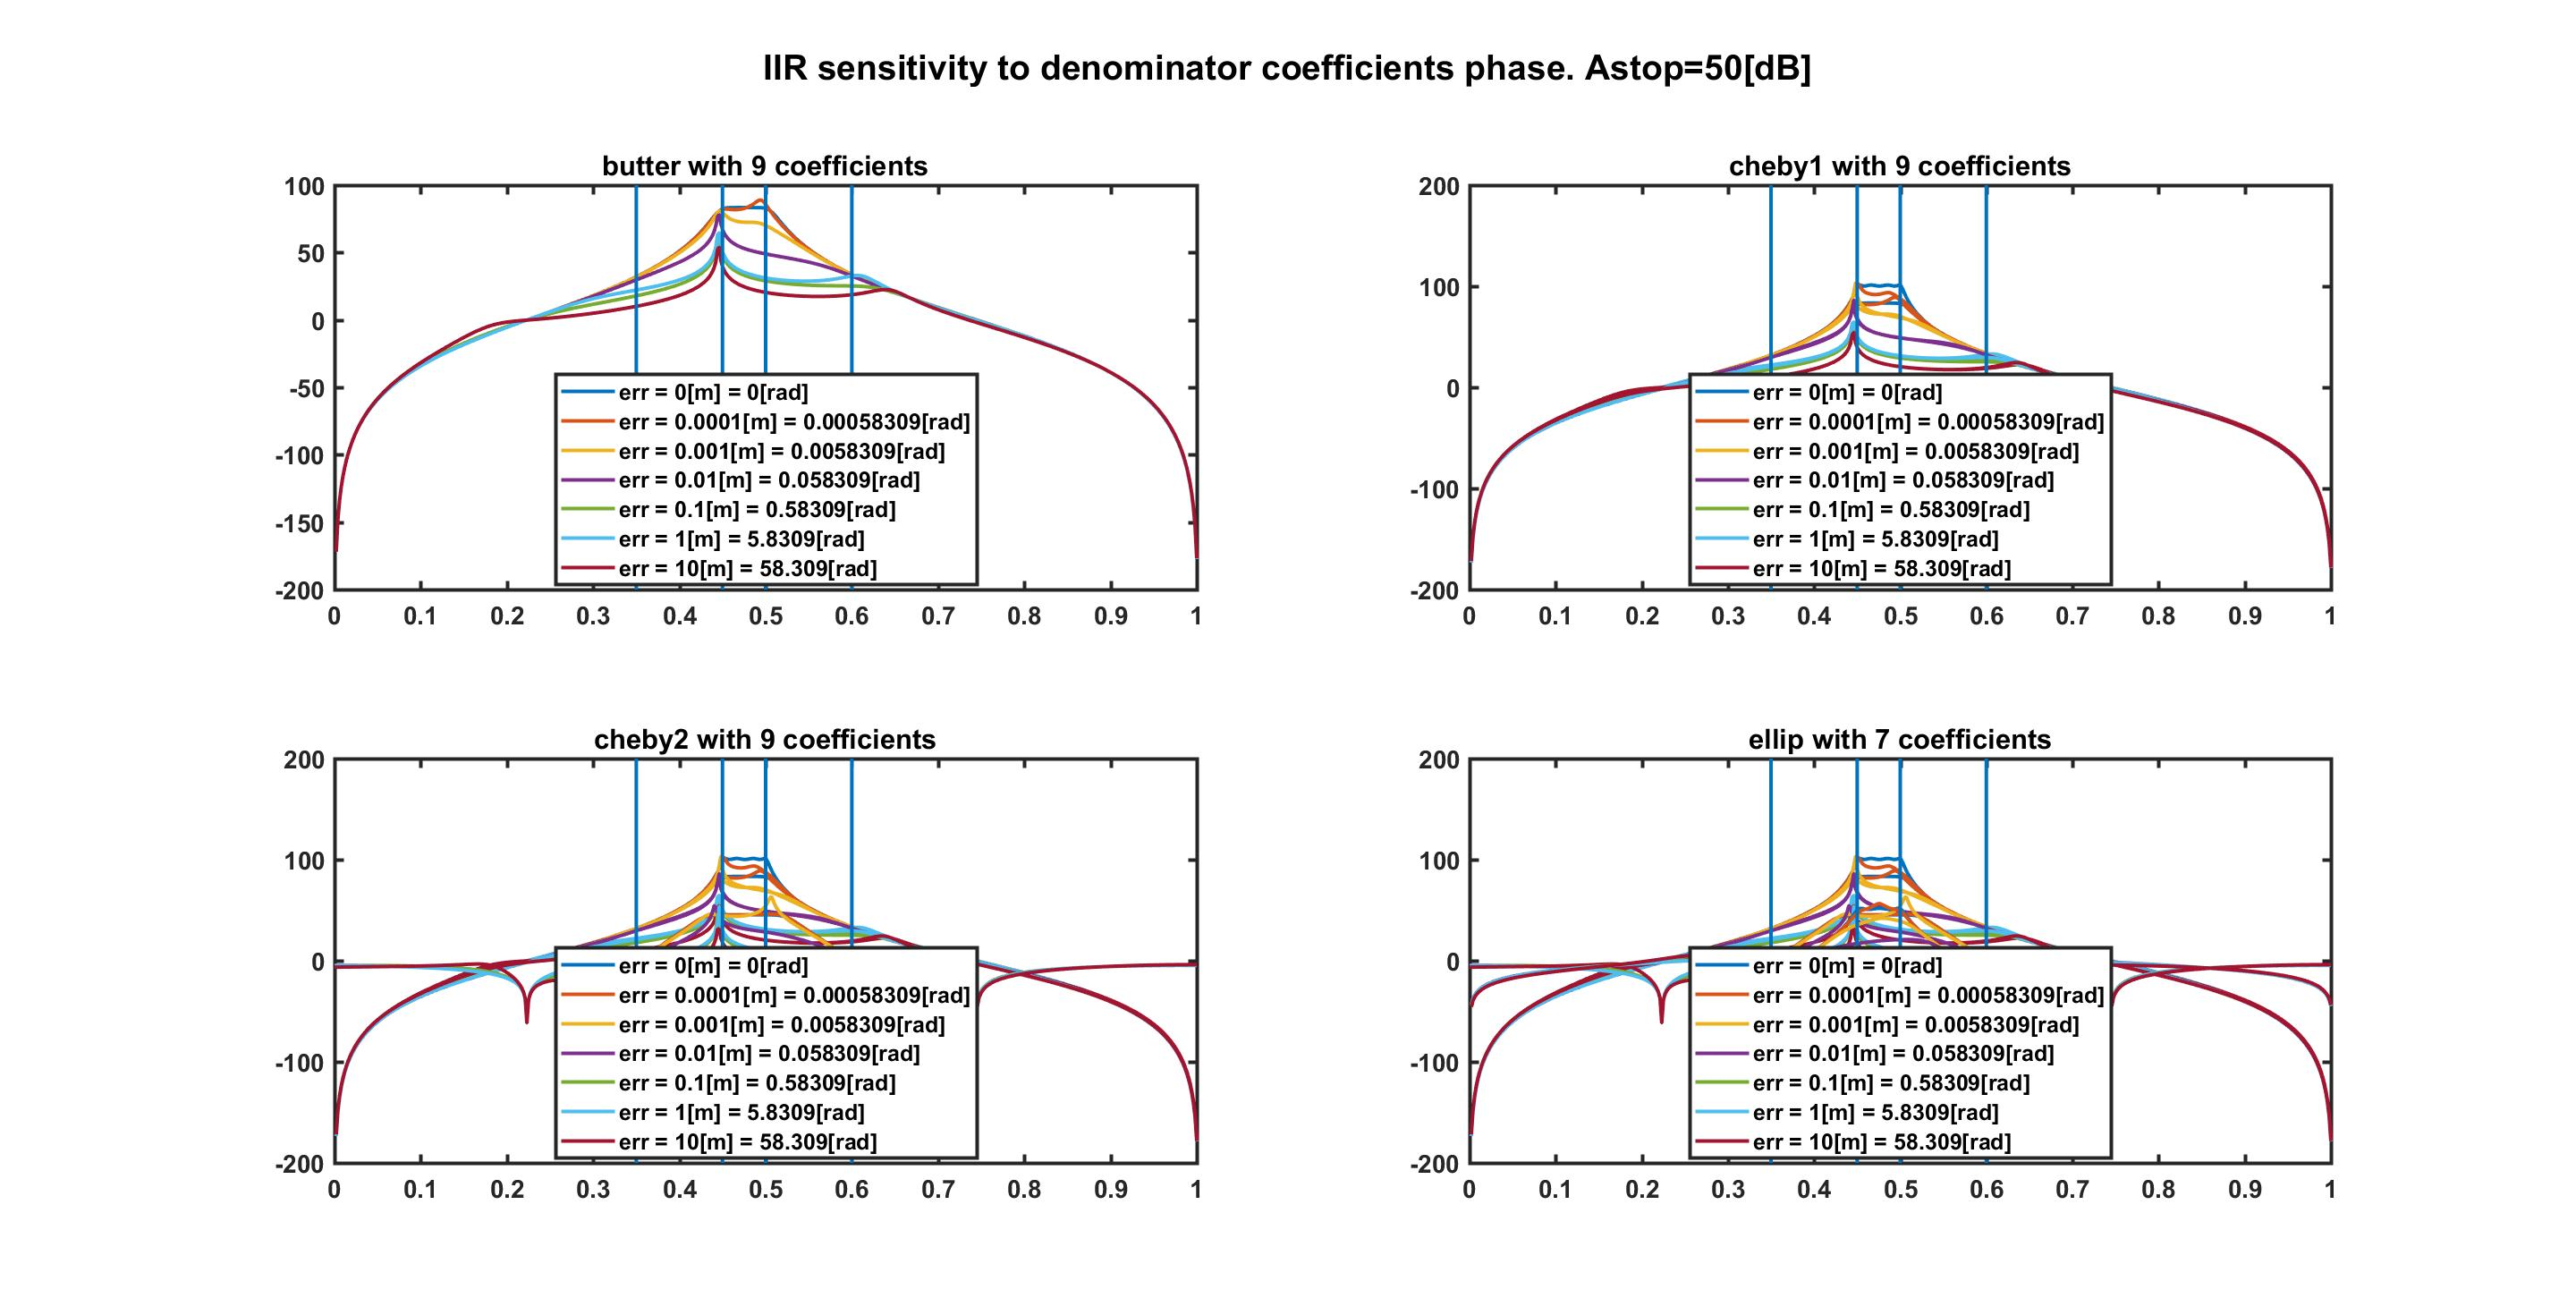
\includegraphics[width=1\textwidth]{Media/filterSensitivitySim/filtSensitivity50dB.jpg}
\end{center}
\label{fig:filtPhaseSensitivity50dB}
\end{figure}
considering a typical acoustic-scenario case of $ c=343_{\frac{m}{s}} $, signal carrier of $ 2_{Khz} $ and an uncertainty of $ 1_{m} $ in the object range estimation, it results in $ \omega\tau_{pd,error} = 2\pi*2*10^{3}\frac{1}{343} = 36_{radians} $ which basically means that the unknown phase is a uniformly distributed stochastic variable in the range of $ \left[0, 2\pi\right) $. To demonstrate the filter sensitivity, we tried 4 filter designs and added the error phase in their denominator (fig.\ref{fig:filtPhaseSensitivity50dB}).

\subsection*{omni-directional feedback implications}

Though for now we want to fully solve the single-speaker scenario, an issue that should be considered in the context of multiple-speaker scenario is the omni-directional feedback transmitter. Heuristically, one can imagine that a signal originated in one speaker (which is not the currently wanted speaker), is fed-back through all the transponders. Among them the wanted speaker also reflects the unwanted signal towards the receiver thus unwontedly enhancing it.
//
Considering $ S $ speakers, the system's transfer function is 
$$
y_{\theta}^{\mathcal{F}}(\omega) 
=
\sum_{s=1}^{S}
{
\frac
{
\vecnot{\alpha}^{T}
\vecnot{d}_{\theta_{s}}
e^{-j\omega\tau_{pd,s}}
}
{
1
-
\sum_{r=1}^{S}
{
\vecnot{\beta}^{T}\vecnot{d}_{\theta_{r}}
e^{-j\omega (\tau_{pd,r}+\tau_{tx,r})}
}
}
x_{s}^{\mathcal{F}}(\omega)
}
$$ 
which can be viewed as a sum of same-non-uniform-denominator (of $ SN $ coefficients with only $ N $ DOFs) transfer functions. The denominator is not uniform because different steering vectors ( $ \vecnot{d}_{theta,s} $ ) represent spatial non-uniform sampling intervals. It can be Heuristically viewed as a polynomial of non-integer powers.  

\section*{Attempts of solving issues}

Initially, our main focus was to solve the sensitivity issues in the single speaker scenario. 

\subsection*{High sensitivity to object range uncertainty}

\subsubsection*{Robust filter design}

We tried to find a filter-design scheme which will generate a robust-to-input-error system. We investigated a few options in this field of solutions.

\textbf{Low sensitivity to coefficients error design}
\\
After thoroughly investigating the subject and reading some interesting articles \cite{Agarwal1975NewNoise,Li1993RoundoffRealizations,Kauraniemi1998DeltaFilters}, we understood that this is not the wanted solution.
\\
In those articles, the main idea was to process the signal around $ z=1 $ instead of $ z=0 $. This enables lower coefficient error sensitivity for cases of close-to-unit-circle poles. The authors introduce a general representation of a second order recursive section. Assuming poles at $ p_{1,2} = r\cos{\theta} \pm jr\sin{\theta} $, $ H(z) = \frac{1}{z^{2}-az+b} $, where $ a = 2r\cos{\theta} $ and $ b = r^{2} $. Their test-case is obviously poles that are close to $ z=1 $, i.e. $ z \approx 1-\alpha T \pm j\beta T $ where $ T $ is the sampling interval, $ \alpha = 1-r, \beta T \approx \theta $ and they also introduced $ \delta = \alpha T $. The $ T $ is mentioned due to the fact that the filter design starts in the $ s $-domain and $ z=e^{sT} $.
\\
Their solution is based on $ sT \rightarrow 0 $ which leads to first-order-taylor approximation $ z \approx 1+sT $. They suggest realizing the IIR section around $ z=1 $ instead of $ z=0 $ by introducing $ \hat{z} = z-1 \approx sT $ which leads to $ \hat{H}\left(\hat{z}\right) = H\left( \hat{z}+1 \right) = \frac{1}{\hat{z}^{2}+\hat{a}z+\hat{b}} $ where $ \hat{a} \approx 2\delta+\theta^{2} $ and $ \hat{b} = \delta^2 + \theta^2 $. 
\\
To implement the filter, they used an integrator for $ \hat{z}^{-1} $.
\\
Not only that we cannot implement a spatial integrator, it doesn't solve our issue but only enables an addition of stochastic noise  to the coefficients values.
Our problem is the only one component of the denominator is noised, the other is just $ 1 $.
\\
\textbf{Solving an optimization problem}
\\
We can formulate the next minimization problem 
\begin{equation*}
\begin{aligned}
& \underset{\vecnot{\alpha},\vecnot{\beta}}{\text{minimize}}
& & 
\left\lVert 
H_{d}(\theta) - H_{\vecnot{\alpha},\vecnot{\beta},\phi}(\theta)
\right\rVert^p
\\
& \text{subject to}
& & 0 < \phi \leq 2\pi, \; i = 1, \ldots, m.
\end{aligned}
\end{equation*}
where 
$ 
H_{\vecnot{\alpha},\vecnot{\beta},\phi}(\theta) =  
\frac
{
\vecnot{\alpha}^{T}
\vecnot{d}_{\theta}
}
{
1
-
\vecnot{\beta}^{T}\vecnot{d}_{\theta}
e^{-j\phi}
}
$
and 
$ 
H_{d}(\theta) =  
\frac
{
\vecnot{\alpha_{d}}^{T}
\vecnot{d}_{\theta}
}
{
\vecnot{\beta}_{d}^{T}\vecnot{d}_{\theta}
}
$
. 
An easy way of modeling the problem is to use the polar ($\vecnot{r_{\vecnot{\alpha},\vecnot{\beta}}},\vecnot{\phi_{\vecnot{\alpha},\vecnot{\beta}}}$) representation of both zeros and poles (which still leaves $ 2N $ DOF) and coefficients.
\\
An initial evaluation was made trying to solve the optimization problem 
\begin{equation*}
\begin{aligned}
& \underset{\vecnot{\alpha},\vecnot{\beta}}{\text{minimize}}
& & 
\left\lVert 
H_{d}(\theta) - H_{\vecnot{\alpha},\vecnot{\beta},\phi}(\theta)
\right\rVert^2
\\
& \text{subject to}
& & 0 < \phi \leq 2\pi, \; i = 1, \ldots, m.
\end{aligned}
\end{equation*}
\begin{figure}[!ht]
\begin{center}

\includegraphics[width=0.3\textwidth]{Media/addPhotoHere.PNG}
\caption
{
The failing attempts of the optimization approach
}
\label{fig:filtOptimizationFail}
\end{center}
\end{figure}
by letting the radius $ r $ and azimuth $ \phi $ of both poles and zeros to be freely modified, thus enabling the filter to have complex coefficients. So far it didn't succeed (fig.\ref{fig:filtOptimizationFail}) and we are not sure that the problem is convex.
\\
Tsvi suggested modifying the optimization criterion to $ \left\lVert \right\rVert^\infty $ and maybe use a weighted version of the problem 
\begin{equation*}
\begin{aligned}
& \underset{\vecnot{\alpha},\vecnot{\beta}}{\text{minimize}}
& & 
\left\lVert 
\left(H_{d}(\theta) - H_{\vecnot{\alpha},\vecnot{\beta},\phi}(\theta)\right)^{T}\vecnot{w}
\right\rVert^\infty
\\
& \text{subject to}
& & 0 < \phi \leq 2\pi, \; i = 1, \ldots, m.
\end{aligned}
\end{equation*}

\subsubsection*{Synthetic sync signal broadcast}

The idea is to insert a synthetic signal of constant frequency to the system. By iteratively modifying the phases of the feedback coefficient, we predict that once we hit the right phase the receiver output energy will be maximal and we can use counter-gradient iterative methods (e.g. newton raphson etc.). Currently (2018 Jan 16th) we are in final stages of creating the simulation of this method.

\subsubsection*{Adapting control theory methods}

An interesting problem in control theory is the ``Networked Controlled System'' which models scenarios of control-via-network where the sensor delay is random (influenced by the network arbitration). Those articles also deal with random data dropouts which are not relevant in our case. Some interesting papers \cite{Luan2011StabilizationDelays,Lewis1998ControlDelays} deal with such problem and we intend to thoroughly read them hoping to adjust their solutions to our case.

\subsection*{omni-directional feedback implications}

Though not our current focus, an interesting idea for solving this issue is implementing a directional ``retro'' feedback which flips the spatial order of the feedback, thus creating a directional feedback that simultaneously transmits to each source only its own feedback signal. 

\clearpage
\small
{
\bibliographystyle{unsrt}
\bibliography{./Modules/Mendeley,./Modules/LocalBib}
}
\end{document}